\subsection{Design and implement a database framework
%a query language and implement a database management 
%system 
that accommodate identified variations}
\label{sec:ro2}

Having an encoding that represent variation we need to incorporate it within the 
database and the query language to allow explicit storing and manipulation of 
variation in a database. Objective 2 aims to design and implement a database framework
that encodes variation directly.
% for a variational
%database and variational query language and implement them as 
%a variational database management system that allows users to interact with a
%variational database. 
\tabref{ro2} presents individual research questions we need
to answer for this objective. 

\begin{table}[H]
\caption{Objective 2 research questions.}
\label{tab:ro2}
\centering
\begin{tabularx}{\textwidth}{X}
\toprule
 \textbf{Objective 2: Design and implement a database framework
%  a query language and implement a database management 
%system 
that accommodates identified variations}
\tabularnewline
\midrule
RQ2.1: How should variation in form of feature expression be incorporated in the database directly? (\dbpl, \poly)
\tabularnewline[0.2cm]
RQ2.2: What are appropriate query languages to interact with a database that accounts for variation explicitly? And how should variation in form of feature expression be incorporated in the query language? (\dbpl, \poly)
\tabularnewline[0.2cm]
RQ2.3: Having a theoretical database framework that accounts for variation explicitly, how 
should we implement a database management system that uses that framework? (In progress)
\tabularnewline
\bottomrule
\end{tabularx}
\end{table}


\begin{comment}
* annotations and choices
\end{comment}

For RQ2.1 we annotate elements of a database with feature expression.
%as introduced in \secref{encode-var}. 
We use annotated elements both in the schema and content.
Within a schema we allow attributes and relations to exist 
conditionally based on the feature expression assigned to them, called \emph{variational schema}.
\secref{vsch} provides the formal definition of variational schema and examples of it.
At the content level, we annotate each tuple with a feature expression, indicating when the tuple 
is present, called \emph{variational table}.
\secref{vtab} provides the formal definition and examples of variational table
which uses \emph{variational sets}, introduced in \secref{v-set}, for the formalizations.
%
Together variational schema and a set of variational tables associated with the 
variational schema create a \emph{variational database (VDB)}, defined in \secref{vtab}.
Conceptually, a  \emph{single} variational database represents \emph{many}
different plain relational
databases, each one corresponding to a different variant of a software system,
\emph{at the same time}.



\begin{comment}
The variational nature of a VDB requires a query language that
accounts for variation directly.
To express and represent variation in queries,
we incorporate choice calculus~\cite{Walk13thesis, EW11tosem}  into a 
structured query language. We formally define 
\emph{variational relational algebra (VRA)} in \secref{vrel-alg}
as our algebraic query language.
A query written in VRA is called a \emph{variational query (v-query)};
when it is clear from context we use query and v-query interchangeably. 
A v-query typically conveys the same intent over several 
relational database variants, however, a single v-query is also capable of capturing different 
intents over different database variants.
Consequently, the expressiveness of v-queries may cause them to be 
more complicated than relational queries, discussed in \secref{type-sys}. 
Hence, we introduce a 
\emph{type system} for VRA that statically checks if a 
v-query conforms to the underlying v-schema and encoded variability within the VDB.
Finally, we close out this section by providing a set of rules in \secref{var-min} 
for reducing a query's variation.

\end{comment}

For RQ2.2 we need to design a query language that reflects the variational 
information need while working with a variational database. 
To express and represent variation in queries,
we incorporate formula choice calculus~\cite{HW16fosd}  into a 
structured query language. We formally define 
\emph{variational relational algebra (VRA)} in \secref{vrel-alg}
as our algebraic query language.
A query written in VRA is called a \emph{variational query (v-query)};
when it is clear from context we use query and v-query interchangeably. 
A v-query typically conveys the same intent over several 
relational database variants, however, a single v-query is also capable of capturing different 
intents over different database variants.


For RQ2.3 and to interact with VDBs using v-queries, we are implementing
and optimizing
\emph{Variational Database Management System (VDBMS)}.
VDBMS is implemented in Haskell. VDBMS sit on 
top of any DBMS that the user desires and used to store their data 
%\arashComment{I did not find any explanation on how v-tables are stored in an RDBMS.} 
%\resp{it is exactly implemented as formalized in v-table section.}
%\responded
in form of variational tables.
%, explained in \secref{vtab}.
%To acquire an extensible system we implement 
To support running VDBMS with multiple different plain relational DBMS backends,
we provide
a shared interface
for connecting to and inquiring information from a DBMS and
instantiate it for different database engines such as PostgreSQL and
MySQL. 
%\rewrite{any dbms that has a library in haskell that has a function
%that returns the result to the user. eg that doesn't satisfy this is 
%database.sqlite3. } --> The following addresses this:
An expert can extend VDBMS to another database engine by
writing methods for connecting to and querying from the database.
\secref{impl} provides details of our implementation and the architectur of 
VDBMS.

\secref{ro3} discusses the objective 3 and its research questions.

\section{Annotations and Variational Sets}
\label{sec:vset}


%\point{annotating elements of database with feature expressions.}
We now introduce the first approach used to incorporate variation into a database.
To incorporate feature expressions into the database,
we \emph{annotate} database elements (including attributes, relations, and tuples) 
with feature expressions. An \emph{annotated element} \elem\ with feature expression \dimMeta\
is denoted by \annot \elem, 
that is, if \elem\ has type \typevar\ (i.e., $\elem \in \typevar$)
then $\annot \elem$ has the corresponding variational type 
$\vartype \typevar$ (i.e., $\annot \elem \in \vartype \typevar$).
%The feature expression \dimMeta\ represents
%the set of configurations where their variants contain element \elem\ because
%
The feature expression attached to an element is called its \emph{presence
condition} since it determines the condition (set of configurations) under
which the element is present in the database. 
This is done by the \emph{configuration} function $\xeSem [] . : \elemSet \totype \confSet \totype \maybe {\pelemSet}$ defined in \figref{vset}.
For example, assuming
$\features=\set{\A,\B}$, the annotated number $\annot [\A \vee \B] 2$ is present
in variants \setDef{\A} (i.e., $\xeSem [\setDef{\A}] {\annot [\A \vee \B] 2}$ = 2), 
\setDef{\B} (i.e., $\xeSem [\setDef{\A}] {\annot [\A \vee \B] 2}$ = 2), 
and \setDef{\A,\B} (i.e.,$\xeSem [\setDef{\A, \B}] {\annot [\A \vee \B] 2} = 2$) 
but not in variant
\setDef{} (i.e., $\xeSem [\setDef { }] {\annot [\A \vee \B] 2} = \bot$). 
%
The operation $\getPC{\annot{\elem}}=e$ returns the presence condition of an
annotated element.
% with a configuration
%that enables either $\A$ or $\B$ or both
%variants that disable both $\A$ and $\B$.
% Here, $\getPC {\annot [\A \vee \B] 2} = \A \vee \B$.

\section{Annotations and Variational Sets}
\label{sec:vset}


%\point{annotating elements of database with feature expressions.}
We now introduce the first approach used to incorporate variation into a database.
To incorporate feature expressions into the database,
we \emph{annotate} database elements (including attributes, relations, and tuples) 
with feature expressions. An \emph{annotated element} \elem\ with feature expression \dimMeta\
is denoted by \annot \elem, 
that is, if \elem\ has type \typevar\ (i.e., $\elem \in \typevar$)
then $\annot \elem$ has the corresponding variational type 
$\vartype \typevar$ (i.e., $\annot \elem \in \vartype \typevar$).
%The feature expression \dimMeta\ represents
%the set of configurations where their variants contain element \elem\ because
%
The feature expression attached to an element is called its \emph{presence
condition} since it determines the condition (set of configurations) under
which the element is present in the database. 
This is done by the \emph{configuration} function $\xeSem [] . : \elemSet \totype \confSet \totype \maybe {\pelemSet}$ defined in \figref{vset}.
For example, assuming
$\features=\set{\A,\B}$, the annotated number $\annot [\A \vee \B] 2$ is present
in variants \setDef{\A} (i.e., $\xeSem [\setDef{\A}] {\annot [\A \vee \B] 2}$ = 2), 
\setDef{\B} (i.e., $\xeSem [\setDef{\A}] {\annot [\A \vee \B] 2}$ = 2), 
and \setDef{\A,\B} (i.e.,$\xeSem [\setDef{\A, \B}] {\annot [\A \vee \B] 2} = 2$) 
but not in variant
\setDef{} (i.e., $\xeSem [\setDef { }] {\annot [\A \vee \B] 2} = \bot$). 
%
The operation $\getPC{\annot{\elem}}=e$ returns the presence condition of an
annotated element.
% with a configuration
%that enables either $\A$ or $\B$ or both
%variants that disable both $\A$ and $\B$.
% Here, $\getPC {\annot [\A \vee \B] 2} = \A \vee \B$.

\section{Annotations and Variational Sets}
\label{sec:vset}


%\point{annotating elements of database with feature expressions.}
We now introduce the first approach used to incorporate variation into a database.
To incorporate feature expressions into the database,
we \emph{annotate} database elements (including attributes, relations, and tuples) 
with feature expressions. An \emph{annotated element} \elem\ with feature expression \dimMeta\
is denoted by \annot \elem, 
that is, if \elem\ has type \typevar\ (i.e., $\elem \in \typevar$)
then $\annot \elem$ has the corresponding variational type 
$\vartype \typevar$ (i.e., $\annot \elem \in \vartype \typevar$).
%The feature expression \dimMeta\ represents
%the set of configurations where their variants contain element \elem\ because
%
The feature expression attached to an element is called its \emph{presence
condition} since it determines the condition (set of configurations) under
which the element is present in the database. 
This is done by the \emph{configuration} function $\xeSem [] . : \elemSet \totype \confSet \totype \maybe {\pelemSet}$ defined in \figref{vset}.
For example, assuming
$\features=\set{\A,\B}$, the annotated number $\annot [\A \vee \B] 2$ is present
in variants \setDef{\A} (i.e., $\xeSem [\setDef{\A}] {\annot [\A \vee \B] 2}$ = 2), 
\setDef{\B} (i.e., $\xeSem [\setDef{\A}] {\annot [\A \vee \B] 2}$ = 2), 
and \setDef{\A,\B} (i.e.,$\xeSem [\setDef{\A, \B}] {\annot [\A \vee \B] 2} = 2$) 
but not in variant
\setDef{} (i.e., $\xeSem [\setDef { }] {\annot [\A \vee \B] 2} = \bot$). 
%
The operation $\getPC{\annot{\elem}}=e$ returns the presence condition of an
annotated element.
% with a configuration
%that enables either $\A$ or $\B$ or both
%variants that disable both $\A$ and $\B$.
% Here, $\getPC {\annot [\A \vee \B] 2} = \A \vee \B$.

\input{formulas/vset}

%\point{vset.}
A \emph{variational set} (\emph{v-set}) $\vset = \setDef {\annot [\dimMeta_1] {\elem_1},\ldots, \annot [\dimMeta_n] {\elem_n}}$ 
is a set of annotated elements, 
that is,
$\vset \in \vsetSet$~\cite{EWC13fosd,Walk14onward,ATW17dbpl}.
We typically omit the presence condition \t\ in a variational set,
e.g., $\annot [\t] 4 = 4$.
% where the presence condition of elements is satisfiable~\cite{EWC13fosd,Walk14onward,vdb17ATW}. 
%
Conceptually, a variational set represents many different plain sets simultaneously.
These plain sets can be generated by \emph{configuring} a variational set with a configuration.
This is done by the \emph{variational set configuration} function
\ensuremath{\osetSem \vset: \vsetSet \totype \confSet \totype \psetSet}, defined in \figref{vset}.
The configuration function evaluates the presence condition $\dimMeta_i$ of each 
element $\elem_i$ of the variational set with the configuration \config. 
If the evaluation results in \t\ it includes $\elem_i$ in the plain set and otherwise it
does not. \exref{vset-conf} illustrates the configuration of a variational set for all
possible configurations. 
\structure{it'd be nice to have the entire ex in the same page.}

\begin{example}
\label{eg:vset-conf}
Assume we have the feature space $\features = \setDef {\A, \B}$ 
and the variational set $\vset_1 = \setDef {\annot [\A] 2, \annot [\B] 3, 4}$.
$\vset_1$ represents four plain sets:
\begin{alignat*}{1}
\osetSem {\vset_1} &=
\begin{cases}
  \setDef{2,3,4}, & \config = \setDef{\A,\B}\\
  \setDef{2,4}, & \config = \setDef{\A}\\
  \setDef{3,4}, & \config = \setDef{\B}\\
  \setDef{4}, & \config = \setDef { }
\end{cases}
\end{alignat*}
This states that, for example, configuring $\vset_1$ for the variant that enables 
bot \A\ and \B\ (that is, \ensuremath{\A = \t, \B = \t}) results in the plain set
\ensuremath{ \osetSem [\setDef {\A, \B}] {\vset_1} = \setDef {2,3,4} }.
\end{example}

%
%\noindent
Following database notational conventions
we drop the brackets of a variational set when used in database
schema definitions and queries.

%\point{annotated vset.}
A variational set itself can also be annotated with a feature expression.
%
%An \emph{annotated variational set} 
$\annot \vset = \setDef {\annot [\dimMeta_1] {\elem_1},\ldots,\annot [\dimMeta_n] {\elem_n}}^\dimMeta$ is an
\emph{annotated variational set}, 
that is, $\annot \vset \in \annotvsetSet$.
% that it is annotated itself by a \emph{feature expression} \dimMeta.
%We denote an annotated variational set of elements $\elem \in \mathbf{\elemSet}$ with
%\annot \elemSet.
Annotating a variational set with the feature expression \dimMeta\ means that all
elements in the variational set are only present when \dimMeta\ evaluates to \t.
The \emph{normalization} operation $\pushIn {\annot \vset}$ applies this
restriction by pushing it into the presence conditions of the individual
elements:
\ensuremath{
\pushIn {\annot \vset}
= 
\setDef{\annot [\dimMeta_i \wedge \dimMeta] {\elem_i} \myOR 
\annot [\dimMeta_i] \elem_i \in \annot \vset, \sat {\dimMeta_i \wedge \dimMeta}
}}.
%\eric{added that both v-set and annot v-set are of the same type.}
%Thus, we consider both variational sets and annotated variational sets to 
%belong to the set of variational set \vsetSet, that is, we consider them to have the same type. 
Note that both the normalization operation and variational set configuration
are overloaded, that is, they are defined for both variational sets and 
annotated variational sets. 
Also, note that the \emph{normalization} operation also removes elements
with unsatisfiable presence conditions and may also be applied
to an unannotated variational set \vset\ since $\annot[\t]{\vset} = \vset$.
%\ensuremath{
%\vset = \setDef {\annot [\dimMeta_1] \elem_1, \ldots, \annot [\dimMeta_n] \elem_n}}, 
%which is equivalent to the annotated v-set \annot [\t] \vset. Thus,
%\ensuremath{
%\pushIn \vset = \setDef {
%\annot [\dimMeta_i] \elem_i \myOR \annot [\dimMeta_i] \elem_i, \sat {\dimMeta_i}
%}
%}.}
%This restriction
%can be captured by the property:
%$\setDef {\annot [\dimMeta_1] {\elem_1} ,\ldots, \annot [\dimMeta_n] {\elem_n}}^\dimMeta
%\equiv 
%\setDef {\annot [\dimMeta_1 \wedge \dimMeta] {\elem_1},\ldots, \annot [\dimMeta_n \wedge \dimMeta] {\elem_n}}
%$.
%
For example, the annotated variational set
$\vset_1 = \{\annot [\A] 2, \annot [\neg \B] 3, 4, \annot [\C] 5\}^{\A \wedge \B}$
indicates that all the elements of the set can only exist
when both $\A$ and $\B$ are enabled. Thus, normalizing the variational set $\vset_1$
%the set's feature expression
results in
$\{\annot [\A \wedge \B] 2,\annot [\A \wedge \B] 4,\annot [\A \wedge \B \wedge \C] 5\}$. The element $3$ is dropped 
%from the set 
since 
\ensuremath{\neg \sat {\getPCfrom 3 {\vset_1} }},
where
\ensuremath{
{\getPCfrom 3 {\vset_1} } = \neg \B \wedge (\A \wedge \B)}.
%its presence condition is unsatisfiable, i.e., $\neg \sat {\neg \fName_2 \wedge (\fName_1 \wedge \fName_2)}$.
%%
Note that we use the function \getPCfrom \elem {\annot \vset} to 
return the presence condition of a unique variational element within a bigger
variational structure. 
Note that,
without loss of generality, we assume that elements in a variational set
are unique since we can simply disjoin the presence conditions of a repeated 
element, that is, 
\ensuremath{\setDef {\annot [\dimMeta] \elem, \annot [\dimMeta] \elem, \annot [\dimMeta_1] \elem_1, \ldots, \annot [\dimMeta_n] \elem_n} = \setDef {\annot [\dimMeta \vee \VVal \dimMeta] \elem, \annot [\dimMeta_1] \elem_1, \ldots, \annot [\dimMeta_n] \elem_n}}.
% by just referring to the element itself without its
%annotation, i.e., \elem.

In \figref{vset}, we also define several operations, such as union and
intersection, over variational sets; these operations are used in \secref{type-sys}. The
semantics of a variational set operation is equivalent to applying the corresponding
plain set operation to every corresponding variant of the argument variational sets. For
example, the union of two variational sets $\vset_1\cup\vset_2$ should produce a new
variational set $\vset_3$ such that
%
$\forall c\in\confSet.\;
\osetSem{\vset_3} = \osetSem{\vset_1}\,\underline{\cup}\,\osetSem{\vset_2}$,
where $\underline{\cup}$ is the plain set union operation.
%
 This property must hold for all operations over variational sets, that is, for all possible operations, \vsetOp, defined on variational sets the property 
 \ensuremath{
 \Pone: 
 \forall \config \in \confSet. \osetSem {\pushIn {\vset_1} \vsetOp \pushIn {\vset_2}} 
 = \osetSem {\vset_1} \psetOp \osetSem {\vset_2}
 } must hold, where \psetOp\ is the counterpart operation on plain sets.%
\footnote{This property is proved for the operations we define over variational sets in Coq proof assistant~\cite{Khan21}.}



%\point{vset.}
A \emph{variational set} (\emph{v-set}) $\vset = \setDef {\annot [\dimMeta_1] {\elem_1},\ldots, \annot [\dimMeta_n] {\elem_n}}$ 
is a set of annotated elements, 
that is,
$\vset \in \vsetSet$~\cite{EWC13fosd,Walk14onward,ATW17dbpl}.
We typically omit the presence condition \t\ in a variational set,
e.g., $\annot [\t] 4 = 4$.
% where the presence condition of elements is satisfiable~\cite{EWC13fosd,Walk14onward,vdb17ATW}. 
%
Conceptually, a variational set represents many different plain sets simultaneously.
These plain sets can be generated by \emph{configuring} a variational set with a configuration.
This is done by the \emph{variational set configuration} function
\ensuremath{\osetSem \vset: \vsetSet \totype \confSet \totype \psetSet}, defined in \figref{vset}.
The configuration function evaluates the presence condition $\dimMeta_i$ of each 
element $\elem_i$ of the variational set with the configuration \config. 
If the evaluation results in \t\ it includes $\elem_i$ in the plain set and otherwise it
does not. \exref{vset-conf} illustrates the configuration of a variational set for all
possible configurations. 
\structure{it'd be nice to have the entire ex in the same page.}

\begin{example}
\label{eg:vset-conf}
Assume we have the feature space $\features = \setDef {\A, \B}$ 
and the variational set $\vset_1 = \setDef {\annot [\A] 2, \annot [\B] 3, 4}$.
$\vset_1$ represents four plain sets:
\begin{alignat*}{1}
\osetSem {\vset_1} &=
\begin{cases}
  \setDef{2,3,4}, & \config = \setDef{\A,\B}\\
  \setDef{2,4}, & \config = \setDef{\A}\\
  \setDef{3,4}, & \config = \setDef{\B}\\
  \setDef{4}, & \config = \setDef { }
\end{cases}
\end{alignat*}
This states that, for example, configuring $\vset_1$ for the variant that enables 
bot \A\ and \B\ (that is, \ensuremath{\A = \t, \B = \t}) results in the plain set
\ensuremath{ \osetSem [\setDef {\A, \B}] {\vset_1} = \setDef {2,3,4} }.
\end{example}

%
%\noindent
Following database notational conventions
we drop the brackets of a variational set when used in database
schema definitions and queries.

%\point{annotated vset.}
A variational set itself can also be annotated with a feature expression.
%
%An \emph{annotated variational set} 
$\annot \vset = \setDef {\annot [\dimMeta_1] {\elem_1},\ldots,\annot [\dimMeta_n] {\elem_n}}^\dimMeta$ is an
\emph{annotated variational set}, 
that is, $\annot \vset \in \annotvsetSet$.
% that it is annotated itself by a \emph{feature expression} \dimMeta.
%We denote an annotated variational set of elements $\elem \in \mathbf{\elemSet}$ with
%\annot \elemSet.
Annotating a variational set with the feature expression \dimMeta\ means that all
elements in the variational set are only present when \dimMeta\ evaluates to \t.
The \emph{normalization} operation $\pushIn {\annot \vset}$ applies this
restriction by pushing it into the presence conditions of the individual
elements:
\ensuremath{
\pushIn {\annot \vset}
= 
\setDef{\annot [\dimMeta_i \wedge \dimMeta] {\elem_i} \myOR 
\annot [\dimMeta_i] \elem_i \in \annot \vset, \sat {\dimMeta_i \wedge \dimMeta}
}}.
%\eric{added that both v-set and annot v-set are of the same type.}
%Thus, we consider both variational sets and annotated variational sets to 
%belong to the set of variational set \vsetSet, that is, we consider them to have the same type. 
Note that both the normalization operation and variational set configuration
are overloaded, that is, they are defined for both variational sets and 
annotated variational sets. 
Also, note that the \emph{normalization} operation also removes elements
with unsatisfiable presence conditions and may also be applied
to an unannotated variational set \vset\ since $\annot[\t]{\vset} = \vset$.
%\ensuremath{
%\vset = \setDef {\annot [\dimMeta_1] \elem_1, \ldots, \annot [\dimMeta_n] \elem_n}}, 
%which is equivalent to the annotated v-set \annot [\t] \vset. Thus,
%\ensuremath{
%\pushIn \vset = \setDef {
%\annot [\dimMeta_i] \elem_i \myOR \annot [\dimMeta_i] \elem_i, \sat {\dimMeta_i}
%}
%}.}
%This restriction
%can be captured by the property:
%$\setDef {\annot [\dimMeta_1] {\elem_1} ,\ldots, \annot [\dimMeta_n] {\elem_n}}^\dimMeta
%\equiv 
%\setDef {\annot [\dimMeta_1 \wedge \dimMeta] {\elem_1},\ldots, \annot [\dimMeta_n \wedge \dimMeta] {\elem_n}}
%$.
%
For example, the annotated variational set
$\vset_1 = \{\annot [\A] 2, \annot [\neg \B] 3, 4, \annot [\C] 5\}^{\A \wedge \B}$
indicates that all the elements of the set can only exist
when both $\A$ and $\B$ are enabled. Thus, normalizing the variational set $\vset_1$
%the set's feature expression
results in
$\{\annot [\A \wedge \B] 2,\annot [\A \wedge \B] 4,\annot [\A \wedge \B \wedge \C] 5\}$. The element $3$ is dropped 
%from the set 
since 
\ensuremath{\neg \sat {\getPCfrom 3 {\vset_1} }},
where
\ensuremath{
{\getPCfrom 3 {\vset_1} } = \neg \B \wedge (\A \wedge \B)}.
%its presence condition is unsatisfiable, i.e., $\neg \sat {\neg \fName_2 \wedge (\fName_1 \wedge \fName_2)}$.
%%
Note that we use the function \getPCfrom \elem {\annot \vset} to 
return the presence condition of a unique variational element within a bigger
variational structure. 
Note that,
without loss of generality, we assume that elements in a variational set
are unique since we can simply disjoin the presence conditions of a repeated 
element, that is, 
\ensuremath{\setDef {\annot [\dimMeta] \elem, \annot [\dimMeta] \elem, \annot [\dimMeta_1] \elem_1, \ldots, \annot [\dimMeta_n] \elem_n} = \setDef {\annot [\dimMeta \vee \VVal \dimMeta] \elem, \annot [\dimMeta_1] \elem_1, \ldots, \annot [\dimMeta_n] \elem_n}}.
% by just referring to the element itself without its
%annotation, i.e., \elem.

In \figref{vset}, we also define several operations, such as union and
intersection, over variational sets; these operations are used in \secref{type-sys}. The
semantics of a variational set operation is equivalent to applying the corresponding
plain set operation to every corresponding variant of the argument variational sets. For
example, the union of two variational sets $\vset_1\cup\vset_2$ should produce a new
variational set $\vset_3$ such that
%
$\forall c\in\confSet.\;
\osetSem{\vset_3} = \osetSem{\vset_1}\,\underline{\cup}\,\osetSem{\vset_2}$,
where $\underline{\cup}$ is the plain set union operation.
%
 This property must hold for all operations over variational sets, that is, for all possible operations, \vsetOp, defined on variational sets the property 
 \ensuremath{
 \Pone: 
 \forall \config \in \confSet. \osetSem {\pushIn {\vset_1} \vsetOp \pushIn {\vset_2}} 
 = \osetSem {\vset_1} \psetOp \osetSem {\vset_2}
 } must hold, where \psetOp\ is the counterpart operation on plain sets.%
\footnote{This property is proved for the operations we define over variational sets in Coq proof assistant~\cite{Khan21}.}



%\point{vset.}
A \emph{variational set} (\emph{v-set}) $\vset = \setDef {\annot [\dimMeta_1] {\elem_1},\ldots, \annot [\dimMeta_n] {\elem_n}}$ 
is a set of annotated elements, 
that is,
$\vset \in \vsetSet$~\cite{EWC13fosd,Walk14onward,ATW17dbpl}.
We typically omit the presence condition \t\ in a variational set,
e.g., $\annot [\t] 4 = 4$.
% where the presence condition of elements is satisfiable~\cite{EWC13fosd,Walk14onward,vdb17ATW}. 
%
Conceptually, a variational set represents many different plain sets simultaneously.
These plain sets can be generated by \emph{configuring} a variational set with a configuration.
This is done by the \emph{variational set configuration} function
\ensuremath{\osetSem \vset: \vsetSet \totype \confSet \totype \psetSet}, defined in \figref{vset}.
The configuration function evaluates the presence condition $\dimMeta_i$ of each 
element $\elem_i$ of the variational set with the configuration \config. 
If the evaluation results in \t\ it includes $\elem_i$ in the plain set and otherwise it
does not. \exref{vset-conf} illustrates the configuration of a variational set for all
possible configurations. 
\structure{it'd be nice to have the entire ex in the same page.}

\begin{example}
\label{eg:vset-conf}
Assume we have the feature space $\features = \setDef {\A, \B}$ 
and the variational set $\vset_1 = \setDef {\annot [\A] 2, \annot [\B] 3, 4}$.
$\vset_1$ represents four plain sets:
\begin{alignat*}{1}
\osetSem {\vset_1} &=
\begin{cases}
  \setDef{2,3,4}, & \config = \setDef{\A,\B}\\
  \setDef{2,4}, & \config = \setDef{\A}\\
  \setDef{3,4}, & \config = \setDef{\B}\\
  \setDef{4}, & \config = \setDef { }
\end{cases}
\end{alignat*}
This states that, for example, configuring $\vset_1$ for the variant that enables 
bot \A\ and \B\ (that is, \ensuremath{\A = \t, \B = \t}) results in the plain set
\ensuremath{ \osetSem [\setDef {\A, \B}] {\vset_1} = \setDef {2,3,4} }.
\end{example}

%
%\noindent
Following database notational conventions
we drop the brackets of a variational set when used in database
schema definitions and queries.

%\point{annotated vset.}
A variational set itself can also be annotated with a feature expression.
%
%An \emph{annotated variational set} 
$\annot \vset = \setDef {\annot [\dimMeta_1] {\elem_1},\ldots,\annot [\dimMeta_n] {\elem_n}}^\dimMeta$ is an
\emph{annotated variational set}, 
that is, $\annot \vset \in \annotvsetSet$.
% that it is annotated itself by a \emph{feature expression} \dimMeta.
%We denote an annotated variational set of elements $\elem \in \mathbf{\elemSet}$ with
%\annot \elemSet.
Annotating a variational set with the feature expression \dimMeta\ means that all
elements in the variational set are only present when \dimMeta\ evaluates to \t.
The \emph{normalization} operation $\pushIn {\annot \vset}$ applies this
restriction by pushing it into the presence conditions of the individual
elements:
\ensuremath{
\pushIn {\annot \vset}
= 
\setDef{\annot [\dimMeta_i \wedge \dimMeta] {\elem_i} \myOR 
\annot [\dimMeta_i] \elem_i \in \annot \vset, \sat {\dimMeta_i \wedge \dimMeta}
}}.
%\eric{added that both v-set and annot v-set are of the same type.}
%Thus, we consider both variational sets and annotated variational sets to 
%belong to the set of variational set \vsetSet, that is, we consider them to have the same type. 
Note that both the normalization operation and variational set configuration
are overloaded, that is, they are defined for both variational sets and 
annotated variational sets. 
Also, note that the \emph{normalization} operation also removes elements
with unsatisfiable presence conditions and may also be applied
to an unannotated variational set \vset\ since $\annot[\t]{\vset} = \vset$.
%\ensuremath{
%\vset = \setDef {\annot [\dimMeta_1] \elem_1, \ldots, \annot [\dimMeta_n] \elem_n}}, 
%which is equivalent to the annotated v-set \annot [\t] \vset. Thus,
%\ensuremath{
%\pushIn \vset = \setDef {
%\annot [\dimMeta_i] \elem_i \myOR \annot [\dimMeta_i] \elem_i, \sat {\dimMeta_i}
%}
%}.}
%This restriction
%can be captured by the property:
%$\setDef {\annot [\dimMeta_1] {\elem_1} ,\ldots, \annot [\dimMeta_n] {\elem_n}}^\dimMeta
%\equiv 
%\setDef {\annot [\dimMeta_1 \wedge \dimMeta] {\elem_1},\ldots, \annot [\dimMeta_n \wedge \dimMeta] {\elem_n}}
%$.
%
For example, the annotated variational set
$\vset_1 = \{\annot [\A] 2, \annot [\neg \B] 3, 4, \annot [\C] 5\}^{\A \wedge \B}$
indicates that all the elements of the set can only exist
when both $\A$ and $\B$ are enabled. Thus, normalizing the variational set $\vset_1$
%the set's feature expression
results in
$\{\annot [\A \wedge \B] 2,\annot [\A \wedge \B] 4,\annot [\A \wedge \B \wedge \C] 5\}$. The element $3$ is dropped 
%from the set 
since 
\ensuremath{\neg \sat {\getPCfrom 3 {\vset_1} }},
where
\ensuremath{
{\getPCfrom 3 {\vset_1} } = \neg \B \wedge (\A \wedge \B)}.
%its presence condition is unsatisfiable, i.e., $\neg \sat {\neg \fName_2 \wedge (\fName_1 \wedge \fName_2)}$.
%%
Note that we use the function \getPCfrom \elem {\annot \vset} to 
return the presence condition of a unique variational element within a bigger
variational structure. 
Note that,
without loss of generality, we assume that elements in a variational set
are unique since we can simply disjoin the presence conditions of a repeated 
element, that is, 
\ensuremath{\setDef {\annot [\dimMeta] \elem, \annot [\dimMeta] \elem, \annot [\dimMeta_1] \elem_1, \ldots, \annot [\dimMeta_n] \elem_n} = \setDef {\annot [\dimMeta \vee \VVal \dimMeta] \elem, \annot [\dimMeta_1] \elem_1, \ldots, \annot [\dimMeta_n] \elem_n}}.
% by just referring to the element itself without its
%annotation, i.e., \elem.

In \figref{vset}, we also define several operations, such as union and
intersection, over variational sets; these operations are used in \secref{type-sys}. The
semantics of a variational set operation is equivalent to applying the corresponding
plain set operation to every corresponding variant of the argument variational sets. For
example, the union of two variational sets $\vset_1\cup\vset_2$ should produce a new
variational set $\vset_3$ such that
%
$\forall c\in\confSet.\;
\osetSem{\vset_3} = \osetSem{\vset_1}\,\underline{\cup}\,\osetSem{\vset_2}$,
where $\underline{\cup}$ is the plain set union operation.
%
 This property must hold for all operations over variational sets, that is, for all possible operations, \vsetOp, defined on variational sets the property 
 \ensuremath{
 \Pone: 
 \forall \config \in \confSet. \osetSem {\pushIn {\vset_1} \vsetOp \pushIn {\vset_2}} 
 = \osetSem {\vset_1} \psetOp \osetSem {\vset_2}
 } must hold, where \psetOp\ is the counterpart operation on plain sets.%
\footnote{This property is proved for the operations we define over variational sets in Coq proof assistant~\cite{Khan21}.}


\begin{table}
\caption[Examples of relation schemas and a variational relation schema]{The relation schema of \empbio\ for variants that enable one of the features \vThree, \vFour, or \vFive\ and the variational relation schema of \empbio\ encompassing 
the three variants of the plain relation \empbio.}
\label{tab:empbio-sch}
\centering
\small
%\footnotesize
%\scriptsize
\begin{subtable}[t]{\textwidth}
\centering
\caption{The relation schema of \empbio\ for variants that enable the feature \vThree.}
\label{tab:empbio-v3}
\begin{tabular} {c | l l l}
%\hline
\multirow{2}{*}{\empbio} & \empno & \sex & \birthdate\\
\cline{2-4}
%\hline
 &12001 & F& 1960-11-06\\
\arrayrulecolor{white}\hline
\end{tabular}
\end{subtable}

\medskip
\medskip
\medskip
\begin{subtable}[t]{\textwidth}
\centering
\caption{The relation schema of \empbio\ for variants that enable the feature \vFour.}
\label{tab:empbio-v4}
\begin{tabular} {c | l l l l}
\multirow{2}{*}{\empbio}  & \empno & \sex & \birthdate & \name\\
\cline{2-5}
 &80001 & M & 1956-09-30 & Nagui Merli \\
\arrayrulecolor{white}\hline
\end{tabular}
\end{subtable}

\medskip
\medskip
\medskip
\begin{subtable}[t]{\textwidth}
\centering
\caption{The relation schema of \empbio\ for variants that enable the feature \vFive.}
\label{tab:empbio-v5}
\begin{tabular} {c | l l l l l}
\multirow{2}{*}{\empbio}  & \empno & \sex & \birthdate & \fname & \lname\\
\cline{2-6}
 & 200000 & M & 1960-01-11 & Selwyn & Koshiba \\
\arrayrulecolor{white}\hline
\end{tabular}
\end{subtable}

\medskip
\medskip
\medskip
\begin{subtable}[t]{\textwidth}
\centering
\footnotesize
\caption{The variational relation schema of \empbio.}
\label{tab:empbio-vsch}
\begin{tabular} {c | l l l l l l l}
%\hline
%\hhline{-==}
\textcolor{blue}{$\vThree \vee \vFour \vee \vFive$} & \textcolor{blue}{\t} & \textcolor{blue}{\t} & \textcolor{blue}{\t} & \textcolor{blue}{$\vFour \wedge \neg \vThree \wedge \neg \vFive$} & \textcolor{blue}{$\vFive \wedge \neg \vThree \wedge \neg \vFour$} & \textcolor{blue}{$\vFive \wedge \neg \vThree \wedge \neg \vFour$}\\
\arrayrulecolor{blue}\hdashline
\multirow{2}{*}{\empbio}  & \empno & \sex & \birthdate & \name & \fname & \lname\\
\arrayrulecolor{black}\cline{2-7}
 &12001 & F& 1960-11-06 & & &  \\
  &80001 & M & 1956-09-30 & Nagui Merli & & \\
   & 200000 & M & 1960-01-11 & & Selwyn & Koshiba \\
\arrayrulecolor{white}\hline
%\job & \titleatt & \salary\\
%\cline{2-3}
%& Assistant Engineer & 61594\\
%& Senior Engineer & 96646\\
%& \ldots & \ldots \\
%& Staff & 77935\\
%& Technique Leader & 58345
\end{tabular}
\end{subtable}

\end{table}

\section{Variational Table}
\label{sec:vtab}

%\TODO{change vdb conf to vtab.}
%\rewrite{read and revise}
%\fromppr{vldb}
%\TODO{remember to use definitions of config elem and vset}
%\TODO{give example of vtab for mot ex}
%%\begin{figure}
%[ht]
%
%\begin{comment}
%\textbf{Relational model generic objects:}
%\begin{syntax}
%%OLD
%D\in \mathbf{Dom} &&& \textit{Domain}\\
%A\in \mathbf{Att} &&& \textit{Attribute Name}\\
%R\in \mathbf{R} &&& \textit{Relation Name}\\
%t \in \mathbf{T} &&& \textit{Tuple}
%\end{syntax}
%
%\medskip
%\textbf{Relational model definition:}
%\begin{syntax}
%l\in \mathbf{L} &=& \vn{A} &\textit{Attribute set}\\
%s \in \mathbb{S} &=& R(A_1, \ldots , A_n ) & \textit{Relation specification}\\
%S \in \mathcal{\mathbf{S}} &\Coloneqq& {\vn{s}} & \textit{Schema}\\
%T \in \mathbf{T} &\Coloneqq& \{\llangle t(1), \ldots, t(k)\rrangle \myOR \\
%&&t(i) \in D_i,
%1 \leq i \leq k ,\\
%&&k = \mathit{arity}(R) \} 
%%v_1^1\in D_1, \ldots, v_n^1\in D_n\rrangle, \ldots, \llangle v_1^m\in D_1, \ldots, v_n^m\in D_n\rrangle|\\
%%&& \hspace{0.5cm} m = \textit{number of } R_I\textit{'s tuples}\} 
%&\textit{Relation Instance (Table)}\\
%%I \in \mathbf{Inst} &\Coloneqq& R_{1_I}, \cdots, R_{n_I} & \textit{Database Instance}
%\end{syntax}
%
%
%\medskip
%\textbf{Variational relational algebra objects:}
%\begin{syntax}
%\synDef \dimMeta \ffSet &&&\textit{Presence condition}\\
%\synDef \vAtt \vAttSet &&&\textit{Variational attribute}\\
%\synDef \vAttList \vAttSet &\eqq& \vAtt, \vAttList \myOR \empAtt &\textit{Variational attribute list}\\
%\synDef \vRelSch \vRelSet &\eqq& \vRelDef &\textit{Variational relation schema}\\
% \vRel &&&\textit{Variational relation}\\
%\synDef \vSch \vSchSet &\eqq& \vSchDef &\textit{Variational schema}\\
% &&&\textit{Variational database instance}
%\end{syntax}
%\end{comment}
%
%%%%%%%%%%%%%%%%%%%%%%%%%%%%%%%%%%%%%%%%%%%%%%%%%%%%
\textbf{Variational database objects:}
\begin{syntax}
%\synDef \vAtt \attNames &&&\textit{Attribute Name}\\
%\synDef \vRel \relNames &&& \textit{Relation Name}\\
%\synDef \vAttList {\boldmth{\mathbf{V} \mathbf{A}}} &\eqq& 
%\setDef {\annot [\dimMeta_1] \vAtt_1, \annot [\dimMeta_2] \vAtt_2, \ldots, \annot [\dimMeta_k] \vAtt_k} & \textit{Variational Set of Attributes}\\
%\synDef \vRelSch \vRelSchSet &\eqq& \vRelDef & \textit{Variational Relation Schema}\\
%\synDef \vSch \vSchSet &\eqq& \vSchDef & \textit{Variational Schema}
%
\synDef \vTuple {\vartype \tupletype} &\eqq& \annot[\dimMeta]{(\vi v \numAtts)} & \textit{Variational Tuple}\\
%\vTuple\in\vRelCont \eqq \annot[\dimMeta_\vTuple]{(\vi v \numAtts)}
\synDef \vRelCont \vRelContSet &\eqq& \setDef {\vi \vTuple \numTuples} & \textit{Variational Relation Content}\\
%\vRelCont \in \vRelContSet \eqq \setDef {\vi \vTuple \numTuples}
\synDef \vTab \tabletype &\eqq& (\vRelSch, \vRelCont) & \textit{Variational Table}\\
\synDef \vdbInst \vdbInstSet &\eqq& \annot [\dimMeta] {\setDef {\vi \vTab \numRels} } & \textit{Variational Database Instance}
%\synDef \vdbInst  \vdbInstSet \eqq \annot [\dimMeta] {\setDef {\vi \vTab \numRels} }
\end{syntax}

\medskip
\textbf{Variational database type synonyms:}
\begin{alignat*}{1}
\vRelContSet &= \settype {(\vartype \tupletype)}\\
\tabletype &= \typepair{\vRelSchSet, \vRelContSet}\\
\vdbInstSet &= \vartype {\left( \settype {\left(\left(\relschtype,\relconttype\right)\right)}\right)}
\end{alignat*}

\medskip
\textbf{Variational tuple configuration:}
%
\begin{alignat*}{1}%\raggedleft
\ouSemType [] . &: {\vartype \tupletype} \to \vRelSchSet \to \confSet \to \maybe \tupletype\\
%\end{flalign*}
%
%\begin{flalign*}%\raggedleft
\ouSem{\vRelSch} {\annot  {\left( {\vi v \numAtts}\right)}}  &\\
& \hspace{-50pt} = \begin{cases}
(v_i, \cdots, v_j), &\If \forall k. 1 \leq i \leq k \leq j \leq l, \fSem {\getPCfrom {\getAtt {k}} \vRelSch \wedge \dimMeta} = \t\\
\bot, &\Otherwise
\end{cases}
%\left( \ovSem {v_1}, \hdots, \ovSem {v_\numAtts} \right) &\\
%& \textit{ where } \forall 1 \leq i \leq \numAtts: \\
%&\hspace{5pt} \ovSem {v_i} = 
%\begin{cases}
%v_i, & \If \fSem {\fModel \wedge \getPC{\getRel{\getAtt{v_i}}} \wedge \getPC {\getAtt {v_i}} \wedge \dimMeta_\tuple} \\
%\varepsilon, & \Otherwise
%\end{cases}
\end{alignat*}

%\medskip
\textbf{Variational relation content configuration:}
%
\begin{alignat*}{1}%\raggedleft
\otSemType [] . &: \vRelContSet \to \vRelSchSet \to \confSet \to \pRelContSet\\
%\end{flalign*}
%
%\begin{flalign*}%\raggedleft
\otSem {\vRelSch} {\setDef {\vi \tuple \numTuples}} &= \setDef {\ouSem {\vRelSch}{\tuple_1}, \hdots, \ouSem{\vRelSch} {\tuple_\numTuples}}
\end{alignat*}

%\medskip
\textbf{VDB instance configuration:}
%
\begin{alignat*}{1}%\raggedleft
\odbSem [] . &: \vdbInstSet \to \confSet \to \pInstSet\\
%\end{flalign*}
%
%\begin{flalign*}%\raggedleft
\odbSem { \annot  {\setDef {\vi \vTab \numRels}}} 
&=\odbSem { \annot  { \setDef {\left( \vRelSch_1, \vRelCont_1\right), \ldots, 
\left( \vRelSch_\numRels, \vRelCont_\numRels\right)}}}\\
& = \begin{cases}
\setDef{\left( \orSem {\vRel_1 \annot [\dimMeta_1 {\wedge \dimMeta}] {\left( \vAttList_1 \right)} }, 
\otSem {\vRelSch_1} {\pushIn {\annot [\dimMeta_1 {\wedge \dimMeta}] \vRelCont_1}} \right), \ldots}, &\If \fSem \dimMeta = \t \\
\setDef {}, \Otherwise
\end{cases}
%&= \setDef {(\orSem {\vRelSch_1}, \otSem {\vRelCont_1}), \hdots, (\orSem {\vRelSch_\numRels}, \otSem {\vRelCont_\numRels} )}&
\end{alignat*}

\caption{VDB instance syntax and configuration.
%The input to all configuration functions assumes a well-formed input,
%either a v-cond (see \secref{type-sys} or a (part of a) VDB.
%\TODO{you need to define well-formedness for vdb and mention it 
%for vcond somewhere in the paper.}
%%V-cond configuration only accepts conditions that are type correct. 
%%All the configuration functions are defined over a given database
%%with v-schema \vSch. 
%A set with question mark at the end, e.g., \maybe \pRelSchSet, 
%denotes an optional type, meaning that the original set is extended
%with a non-value, \ensuremath{\bot}.
%\revised{
Note that the schema of a relation must be passed to the configuration function
for its content,
however, the variational schema does not need to be passed to configuration 
functions of smaller parts of the variational schema such as \orSem .  or \olSem .
since all needed information for configuring a part of a variational schema
is propagated. 
%Note that $\vRelContSet = \settype {(\vartype \tupletype)}$.
%}
% of variational set of attributes, v-relations, and v-schema.
%$\varepsilon$ denotes a non-existent relation and value.
%Note that the feature model and 
%relation presence condition are passed all the way to attributes due to the 
%hierarchal structure of presence conditions within a v-schema.
}
\label{fig:vdb-conf}
\end{figure} 

%
%Variation also exists in database content. To account 
%for content variability, we tag tuples with 
%presence conditions. 
%%e.g., the tuple $(1,2)^{\A}$ only exists
%%when \A\  is enabled. 
%%
%Thus, a \emph{variational tuple} (\emph{v-tuple}) is an annotated tuple,
%$\vTuple\in\vRelCont \eqq \annot[\dimMeta_\vTuple]{(\vi v \numAtts)}$. A
%variational tuple corresponds to a variational relation,
%$\vRel\annot[\dimMeta_\vRel]{(\vi \vAtt \numAtts)}$,
%where each element $v_i$ is a value corresponding to attribute $\vAtt_i$
%(recall that attributes in a variational relation are ordered).
%%
%For example, $\annot[\tFive]{(38, PL, 678)}$ is a variational tuple that belongs to the
%\ecourse\ relation from \exref{vsch} and is only present when \tFive\ is
%enabled. 
%%
%The content of a variational relation
%%  \emph{variational relation content} 
%is a set of variational tuples,
%$\vRelCont \in \vRelContSet \eqq \setDef {\vi \vTuple \numTuples}$
%and 
%%
%a \emph{variational table} (\emph{v-table}) is the pair of its relation
%schema and content, $\vTab = (\vRelSch, \vRelCont)$.
%%
%A \emph{variational database instance}
%%of VDB \vDB\ with variational schema \vSch, 
%is a set of variational tables,
%$\synDef \vdbInst  \vdbInstSet \eqq \annot [\fModel] {\setDef {\vi \vTab \numRels} }$.
%%
%A VDB instance is \emph{well-formed} if its encoded variation at
%the schema and content level are consistent and satisfiable~\cite{ALW21vamos}.
%% We define properties that must hold for a VDB to be well-formed can be 
%% found in~\cite{ALW21vamos}.
%
%
%\NOTE{The explanation in the following two paragraphs is really hard to follow.
%Some ideas for improvement: (1) State the requirement that you're talking about
%first, then explain how VDB satisfies it; currently the requirement comes at
%the end, so for 1--3 sentences the reader is wondering why you're re-hashing
%this aspect of VDB. (2) The reader has forgotten by now what the requirements
%are, so a brief (few words) description is needed for each requirement as you
%discuss it. (3) It would help to follow the same order of requirements as
%\secref{mot} as closely as possible. 
%
%\medskip
%I recommend structuring this discussion more rigidly as, ``This encoding
%satisfies \nZero, which is about foo, by doing bar. It satisfies \nOne, which
%is about blah, by doing baz.'' Obviously there's plenty of room for making it
%read more nicely than that, but the lack of structure is making it hard to
%understand as-is.}
%
%
%This encoding of variational databases satisfies the requirements for a
%variational database described in \secref{mot}. Similar to a variational schema, a user
%can configure a variational table or a VDB for a specific variant, formally defined in
%\figref{vdb-conf} in \appref{vdb-conf}. This allows users to deploy a VDB for a
%specific configuration and generate the corresponding VDB variant, satisfying
%database part of \nThree\ need.
%%
%Additionally, 
%our VDB framework puts all variants of a database into
%one VDB (satisfying \nZero) 
%and it keep tracks of which variant a tuple belongs to by 
%annotating them with presence conditions. 
%For example, consider tuples
%\ensuremath{\annot [\tFive] {(38, PL, 678)}}
%and 
%\ensuremath{\annot [\tFour] {(23, DB, \nul)}}
%that belong to the \ecourse\ table. 
%The presence conditions \tFive\ and \tFour\ state that tuples belong to temporal
%variants four and five of this VDB, respectively.
%Hence, this framework tracks which variants a tuple belongs to 
%(first part of \nTwo).
%
%
%%As shown, o
%Our VDB framework encodes variation in databases 
%at two levels: schema and content.
%% We do not extend variation to 
%%the constraint level and only focus on variation at the schema 
%%and content levels. 
%In a database that is a variational artifact as defined in \secref{req},
%while content-level variation can stand on its own, such as
%frameworks used for database versioning and 
%experimental databases~\cite{dbVersioning},
%the schema level cannot, e.g., 
%\ensuremath{
%\ecourse \left(\cno, \cname, \optAtt [\tFive] [\deptno] \right)^{\edu \wedge \left(\tFour \vee \tFive\right)}
%} encodes variation at the schema level for relation \ecourse.
%Dropping the presence conditions of tuples leads to ambiguity, i.e.,
%it is unclear which variant each of the tuples
%\ensuremath{(38, PL, 678)}
%and 
%\ensuremath{(23, DB, \nul)} belongs to. We can only guess that
%they belong to variants where \tFour\ or \tFive\ are enabled, but, 
%we do not know for sure which one. Thus, it violates the \nTwo\ 
%requirement of a variational database framework.
%%where it is unclear which variant each tuple belongs to
%%and there is no way to recover such information.
%%Note that 
%%the VDB framework encodes both schema- and content-level
%%variation. A simpler framework could be used to encode 
%%only content-level variation (where tables consist of variational tuples but
%%have plain relational schema), similar to frameworks used for 
%%database versioning and experimental databases~\cite{dbVersioning}.
%%However, schema-level variation cannot be encoded without 
%%accounting for content-level variation in a framework where
%%variants coexist in parallel and they are all put into one database,
%%e.g., while 
%%\ensuremath{
%%\ecourse \left(\cno, \cname, \optAtt [\tFive] [\deptno] \right)^{\edu \wedge \left(\tFour \vee \tFive\right)}
%%} encodes variation at the schema-level for relation \ecourse,
%%dropping presence conditions of tuples results in tuples
%%\ensuremath{(38, PL, 678)}
%%and 
%%\ensuremath{(23, DB, \nul)}
%%where it is unclear which variant each tuple belongs to
%%and there is no way to recover such information.
%
%
%Note that we limit the granularity of variation in content to tuples, that is,
%the individual values within a tuple are not variational.
%%
%%Note that the value $v_i$ is present iff 
%%$\sat {\dimMeta_\vTuple \wedge \dimMeta_\vRel \wedge \dimMeta_\vAtt \wedge \fModel}$,
%%where, 
%%$\dimMeta_\vAtt = \getPC {\getAtt i}$ and
%%%,
%%%$\dimMeta_\vTuple = \getPC \vTuple$,
%%%\dimMeta = \getPC \vRel,
%%%and 
%%%\fModel\ is the feature model.
%%%
%%for simplicity, 
%%%Also, note that to avoid overcrowding the database with variation and feature 
%%%expressions
%%we only annotate tuples and not cells. 
%This design decision causes some redundancy.
%For example, the two tuples
%\ensuremath{\annot [\tFive] {(38, PL, 678)}} and 
%\ensuremath{\annot [\neg \tFive] {(38, PL, \nul)}}
%%\ensuremath{\annot [\fOne] {(1,2)}} and \ensuremath{\annot [\neg\fOne] {(1,3)}}
%cannot be represented as a single tuple
%% \ensuremath{(1, \chc [\fOne] {2,3})} 
%with variation in the third element. However, this design decision
%does not prevent us from distinguishing between a \nul\ value
%that represents a missing value and a \nul\ value that represents
%a cell that is not present. This distinction can be made by checking
%the satisfiability of 
%the presence condition of the value $v_i$ in tuple \vTuple\ of relation \vRel\ in schema \vSch:
%If $\sat{\getPCfrom {v_i} \vTuple}$ then the \nul\ indicates a missing value
%and otherwise it indicates a non-present cell, where 
%\ensuremath{\getPCfrom {v_i} \vTuple = \dimMeta_\vTuple \wedge \getPCfrom \vRel \vSch
%\wedge \getPCfrom {\getAtt i} \vRel}.
%% \dimMeta_\vRel \wedge \dimMeta_\vAtt \wedge \fModel
%%\revised{
%%where \ensuremath{\chc [\fOne] {2,3}} is a \emph{choice} of values $2$ and $3$
%%and it states that if \A\ is enabled the cell holds the value $2$ and otherwise it 
%%holds the value $3$. }
%%
%
%%\begin{figure}

%%%%%%%%%%%%%%%%%%%%%%%%%%%%%%%%%%%%%%%%%%%%%%%%%%%
\textbf{Variational Set of Attributes Configuration:}
\begin{flalign*}
& \olSem [] . : \ \vAttSet \to \confSet \to \pAttSet&\\
%\end{flalign*}
%
%\begin{flalign*}
& \olSem {\{\optAtt\} \cup \vAttList} \spcEq  
    \begin{cases}
        \{\pAtt\} \cup \olSem{\vAttList},
                            & \If \fSem {\dimMeta \wedge \getPC{\getRel \vAtt} \wedge \fModel} \\
        \olSem{\vAttList} , & \Otherwise
     \end{cases} &\\
% & \olSem {\{\optAtt\} \cup \vAttList} &\spcEq &\  \olSem {\{\optAtt\}} \cup \olSem {\vAttList}\\
& \olSem {\setDef{}} \spcEq  \setDef{}&
\end{flalign*}

%
\medskip
\textbf{Variational Relation Schema Configuration:}
\begin{flalign*}%\raggedleft
&\orSem [] . : \vRelSchSet \to \confSet \to \pRelSchSet&\\
%\end{flalign*}
%
%\begin{flalign*}
&\orSem \vRelDef = 
	\begin{cases}
		\vRel({\olSem {\vAttList}}, &\If \fSem {\dimMeta \wedge \fModel}) \\
		\empRel, &\Otherwise
	\end{cases}&
\end{flalign*}

%
\medskip
\textbf{Variational Schema Configuration:}
\begin{flalign*}%\raggedleft
&\osSem [] . : \vSchSet \to \confSet \to \pSchSet&\\
%\end{flalign*}
%
%\begin{flalign*}
&\osSem {\annot [\fModel] {\setDef {\vRelDefNum 1, \ldots, \vRelDefNum \numRels}}}
%&\hspace{0.3cm}
= \begin{cases}
%		\setDef {\orSem {\vRelDefNumF 1}, \ldots, \orSem {\vRelDefNumF n}},
                 \setDef {\orSem {\vRel_1( \vAttList_1 )^{\dimMeta_1 \wedge \fModel} }, \ldots, 
                 \orSem {\vRel_\numRels( \vAttList_\numRels)^{\dimMeta_\numRels \wedge \fModel} }},		
        & \If \fSem \fModel \\
        \setDef{}, & \text{otherwise}
	\end{cases}&
\end{flalign*}

\medskip
\textbf{Variational Tuple Configuration:}
%
\begin{flalign*}%\raggedleft
&\ouSem [] . : \vRelCont \to \confSet \to \pRelCont&\\
%\end{flalign*}
%
%\begin{flalign*}%\raggedleft
&\ouSem {\annot [ \dimMeta_\tuple] {\left( {\vi v \numAtts}\right)}} = \left( \ovSem {v_1}, \hdots, \ovSem {v_\numAtts} \right) 
%&\\
& \textit{ where } \forall 1 \leq i \leq \numAtts: 
%&\hspace{5pt} 
\ovSem {v_i} = 
\begin{cases}
v_i, & \If \fSem {\fModel \wedge \getPC{\getRel{\getAtt{v_i}}} \wedge \getPC {\getAtt {v_i}} \wedge \dimMeta_\tuple} \\
\varepsilon, & \Otherwise
\end{cases}
\end{flalign*}

\medskip
\textbf{V-Relation Content Configuration:}
%
\begin{flalign*}%\raggedleft
&\otSem [] . : \vRelContSet \to \confSet \to \pRelContSet&\\
%\end{flalign*}
%
%\begin{flalign*}%\raggedleft
&\otSem {\setDef {\vi \tuple \numTuples}} = \setDef {\ouSem {\tuple_1}, \hdots, \ouSem {\tuple_\numTuples}}&
\end{flalign*}

\medskip
\textbf{VDB Instance Configuration:}
%
\begin{flalign*}%\raggedleft
&\odbSem [] . : \vInstSet \to \confSet \to \pInstSet&\\
%\end{flalign*}
%
%\begin{flalign*}%\raggedleft
&\odbSem { {\setDef {\vi \vTab \numRels}}} = \setDef {(\orSem {\vRelSch_1}, \otSem {\vRelCont_1}), \hdots, (\orSem {\vRelSch_\numRels}, \otSem {\vRelCont_\numRels} )}&
\end{flalign*}

\caption{
V-cond and VDB instance configurations.
% of variational set of attributes, v-relations, and v-schema.
$\varepsilon$ denotes a non-existent relation and value.
%Note that the feature model and 
%relation presence condition are passed all the way to attributes due to the 
%hierarchal structure of presence conditions within a v-schema.
}
\label{fig:vdb-conf}
\end{figure} 


\subsubsection{Variational Relational Algebra}
\label{sec:vrel-alg}


%\point{vra = cc + ra}
%Considering the variational nature of a VDB, to satisfy a user's information 
%need when extracting information, 
%we need a query language that not only considers the structure of 
%relational databases (such as SQL and relational algebra (RA)) but also 
%accounts for the variation encoded in the VDB. We achieve this by:
%1) picking relational algebra as our main query language and
%2) using \emph{choices}~\cite{Walk13thesis, EW11tosem} 
%and presence conditions to account for variation. 

To account for variation, VRA combines relational algebra (RA) with 
\emph{choices}~\cite{Walk13thesis, EW11tosem}.
%\point{choice.}
A choice $\chc{x,y}$ consists of a feature expression \dimMeta\ and 
two alternatives $x$ and $y$. For a given configuration \config, 
the choice $\chc{x, y}$ can be replaced by $x$ if \dimMeta\
evaluates to \t\ under configuration \config, (i.e., \fSem{\dimMeta}),
or $y$ otherwise. 
In essence, choices allow a v-queries
to encode variation in a structured and systematic manner. 

\begin{figure}
\begin{syntax}

\multicolumn{4}{l}{\textbf{Operators:}} \\[1ex]
\bullet
  &\eqq& \multicolumn{2}{l}{< \myOR \leq \myOR = \myOR \neq \myOR > \myOR \geq} \\
\circ
  &\eqq& \cup \myOR \cap \\[2ex]

\multicolumn{4}{l}{\textbf{Variational conditions:}} \\[1ex]
\vCond\in\vCondSet
  &\eqq&  \multicolumn{2}{l}{
          \bTag
   \myOR  \pAtt \bullet \cte
   \myOR  \pAtt \bullet \pAtt
   \myOR  \neg \vCond
   \myOR  \vCond \vee \vCond} \\
  &\myOR& \multicolumn{2}{l}{
          \vCond \wedge \vCond
   \myOR \chc{\vCond,\vCond}} \\[2ex]

\multicolumn{4}{l}{\textbf{Variational queries:}} \\[1ex]
\vQ\in\qSet
  &\eqq&  \vRel     & \textit{Relation}\\
  &\myOR& \vSel \vQ & \textit{Selection}\\
  &\myOR& \vPrj[\vAttList]{\vQ} & \textit{Projection}\\
  &\myOR& \chc{\vQ,\vQ} & \textit{Choice}\\
% &\myOR& \vQ \Join_\vCond \vQ & \textit{Variational Join}\\
  &\myOR& \vQ \times \vQ & \textit{Cartesian Product}\\
  &\myOR& \vQ \circ \vQ  & \textit{Set Operation}\\
% &\myOR& \vQ \backslash \vQ &\textit{Variational Set Difference}\\
  &\myOR& \empRel & \textit{Empty Relation}

\end{syntax}

\caption[Syntax of variational relational algebra]{Syntax of variational relational algebra.}
%\TODO{remember that
%you removed join (also removed it from query config def and constrain query 
%by schema). if you want use it just say it's a syntactic sugar.}
%$<, \leq, =, \neq, >, \geq$.
%$\circ$ denotes set operators: union and difference.}
\label{fig:v-alg-def}
\end{figure}



%\point{explain notation and VRA operations.}
The syntax of VRA is given in \figref{v-alg-def}.
%
In VRA, the selection operation is similar to standard RA selection except
that the condition parameter is \emph{variational} meaning that it may contain
choices.
For example, the query 
\ensuremath{\sigma_{\chc {\vAtt_1=\vAtt_2,\vAtt_1=\vAtt_3}} \vRel}
selects a v-tuple \vTuple\ if it satisfies
the condition \ensuremath{\vAtt_1 = \vAtt_2} 
and  \ensuremath{\sat {\dimMeta \wedge \getPC \vTuple}}
or
if \ensuremath{\vAtt_1 = \vAtt_3} 
and \ensuremath{\sat {\neg \dimMeta \wedge \getPC \vTuple }}.
%
The projection operation is parameterized by a v-set of attributes. For
example,
the query $\pi_{\vAtt_1, \optAtt [\dimMeta] [\vAtt_2]} \vRel$
projects $\vAtt_1$ from relation \vRel\ unconditionally, and $\vAtt_2$ 
when \sat{\dimMeta}.
%
The choice operation enables combining two v-queries to be used in different
variants based on a given feature expression. In practice,
it is often useful to return information in some variants and nothing at all in
others. We introduce an explicit \emph{empty} query \empRel\ to facilitate
this. The empty query is used, for example, in 
\ensuremath{\vQ_2} in \exref{vq-specific}. 
%The set operations between queries are v-set operations defined in \secref{vset}.
The rest of VRA's operations are similar to RA, where all set operations
(union, intersection, and cross product) are changed to the corresponding
variational set operations defined in \secref{vlist-vset}.
%
In examples, we also use a join operation with a variational condition,
$\vQ_1\bowtie_\vCond\vQ_2$, which is syntactic sugar for
$\sigma_\vCond(\vQ_1\times\vQ_2)$.


Our implementation of VRA also provides mechanisms for renaming queries and
qualifying attributes with relation/subquery names. These features are needed
to support self joins and projecting attributes with the same name in different
relations. However, for simplicity, we omit these features from the formal
definition in this proposal.


%A query can simply 
%refer to a relation, filter tuples based on a variational condition 
%(which is a relational condition with choices of two conditions), and
%project a variational list of attributes. Besides production of two queries and
%set operations, VRA allows for a choice of two v-queries. This demands an
%\emph{empty} query since an alternative of a choice can very well inquire 
%no information at all. 
%For example, the query $\chc {\vQ_1, \}$
%

%\subsubsection{Running a V-Query on a VDB Results in a V-Table}
%\label{sec:run-vq-get-vtab}
%A v-query systematically represents a set of relational query variants associated to their
%corresponding database variants. Hence, intuitively the user expects to 
%get such variation in their result as well. 

The result of a v-query is a v-table with the relation name $\mathit{result}$.
%
For example, assume that v-tuples $\annot[\fOne]{(1,2)}$ and $\annot[\neg
f_3]{(3,4)}$ belong to a v-relation $\vRel(\vAtt_1,\vAtt_2)$, which is the only
relation in a VDB with the trivial feature model \t.
%
The query $\chc[f_3]{\pi_{\optAtt[f_2][\vAtt_1]}\vRel,\empRel}$ returns a
v-table with relation schema $\annot[f_3]{\mathit{result}(\annot[f_2]{a_1})}$,
which indicates that the result is only non-empty when $f_3$ is true and that the
result includes attribute $a_1$ when $f_2$ is true. \secref{type-sys} defines a
type system that yields the relation schema for any well-formed query.
%
The content of the result relation is a single v-tuple $\annot[f_1]{(1)}$. The
tuple $\annot[\neg f_3]{(3)}$ is not included since the projection occurs in
the context of the choice in $f_3$, which is incompatible with the presence
condition of the tuple (i.e., $\unsat{f_3 \wedge\neg f_3}$). This illustrates
how choices can effectively filter the tuples in a VDB based on their presence
conditions.

% Although there is no need to update the presence condition of the returned
% tuples, yet choices can filter the returned v-tuples.

% Note that here the value \ensuremath{1}
% of attribute \ensuremath{\vAtt_1} is present in VDB variants where 
% \ensuremath{\sat {\A \wedge \B \wedge \C}} although the presence 
% condition of the returned v-tuple does not have to state this condition
% since 
%
% overall presence 
%condition and the presence conditions of attributes and tuples are
%restricted by the variation enforced by the query.
%
%Note that the presence condition of tuples, attributes, and the return relation
%is restricted by the variation enforced by the query. 
% correct this so that you don't conjunct the pc of relation and clarify that it's relations's pc and not the attributes. although the conjunction should be satisfiable.}
%




%%Hence, VRA is more expressive than RA 
%%because it can encode variational queries.
%The variational nature allows users to write interesting queries in many ways:
%1) to express their variational information need or to filter returned tuples
%they can use annotations or 
%choices, \exref{vq-specific},
%2) to express the same intent over several database variants they can 
%use choices in queries or conditions, \exref{vq-same-intent-mult-vars},
%and 
%3) they can also use choices to express different intents over database variants.
%\TODO{Eric, should we drop the last since it creates messy results and isn't really useful?}.
%%The expressiveness of VRA satisfies \textbf{N1}, this is illustrated in 
%%\exref{vq-specific} and \exref{vq-same-intent-mult-vars}.
%%Interestingly, VRA's expressiveness enables users to express 
%%their information need more specifically by stating the exact condition
%%under which an information need is inquired. \exref{vq-specific} illustrates this.
%%It also allows users to express the same intent over several database 
%%variants

% \NOTE{
% To express the variational information need or to filter returned tuples
% users can use annotations or choices. \exref{vq-specific} illustrates this.
% }

The following example illustrates, in the context of our running example, how
a v-query can be used to express variational information needs.

\begin{example}
\label{eg:vq-specific}
%VRA's expressiveness consequently facilitates expressing exactly the condition
%under which an information need is inquired. 
Assume a VDB with
features \vThree, \vFour, and \vFive, and
the corresponding \empbio\ schema variants in \tabref{mot}. 
The v-schema for this VDB is:
%
\begin{align*}
\vSch_2 &=
\{\empbio (\empno, \sex, \birthdate,
\optAtt [\vFour] [\name], \optAtt [\vFive] [\fname],
%& \hspace{16pt} 
\optAtt [\vFive] [\lname] )\}^{\fModel_2}\\
& \hspace{4pt} \textit{where } \fModel_2 = {\vThree \oplus \vFour \oplus \vFive}.
%\left(\vThree \wedge \neg \vFour \wedge \neg \vFive\right)
%  \vee \left(\vFour \wedge \neg \vThree \wedge \neg \vFive\right) 
%   \vee \left(\vFive \wedge \neg \vThree \wedge \neg \vFour\right)}.
\end{align*}
%
The user wants the employee ID numbers (\empno) and names for variants 
\vFour\ and \vFive.
The user needs to project the \name\ attribute 
for variant \vFour, the \fname\ and \lname\ attributes for variant \vFive,
and \empno\ attribute for both variants.
This can be expressed with the following v-query.
\[
\vQ_1 = \pi_{\optAtt [\vFour \vee \vFive] [\empno], \name, \fname, \lname} \empbio
\]
\end{example}

Note that the user does not need to repeat the variability information encoded
in the v-schema in their query, that is, they do not need to annotate \name,
\fname, and \lname\ with \vFour, \vFive, and \vFive, respectively. We discuss
this in more detail in \secref{type-sys} and \secref{constrain}. $\vQ_1$
queries all three variants simultaneously although the returned results are
only associated with variants \vFour\ and \vFive\ due to the annotation of the
attribute \empno\ in the query and the presence conditions of the rest of the
projected attributes in the schema.
%
Yet, selecting only two out of the three variants can be written more
explicitly in a query by using a choice:
$\vQ_2=\chc[\vFour\vee\vFive]{\pi_{\empno,\name,\fname,\lname}\empbio,\empRel}$. 
%
Note that queries $\vQ_1$ and $\vQ_2$ return the same set of v-tuples since
neither returns tuples associated with variant \vThree, but their returned
v-tables have different presence conditions, as will be discussed later in
\exref{type}. 
%

%\NOTE{
VRA has semantic-preserving equivalence rules that allow users 
to incorporate their taste and preference of where and how
 they want to encode variation in their queries. These rules
 factor out the commonality of subqueries and generate queries
 with less variation. \secref{var-min} expands on these rules.
%}

The next example illustrates how a v-query can be used to express the same
intent over several database variants using choices and conditions. Expressing
the same intent over several instances by a single query relieves the DBA from
maintaining separate queries for different versions or configurations of the
schema.

\begin{example}
\label{eg:vq-same-intent-mult-vars}
Assume a VDB with features \vOne--\vFive\ and the corresponding \basic\ schema
variants in \tabref{mot}. The user wants to get all employee names across all
variants, which they can express by the following v-query.
%
\begin{align*}
\vQ_3 &= 
  \vOne\chcL
    \pi_{\name}\engemp \cup \pi_{\name}\othemp, \\
 & \hspace{18pt}
    (\vTwo\vee\vThree)\chcL
      \pi_{\name}\empacct, 
%      \\
% & \hspace{24pt}
      \chc[(\vFour\vee\vFive)]{\pi_{\name,\fname,\lname}\empbio, \emp}\chcR\chcR
\end{align*}
%
Since the v-schema enforces that exactly one of \vOne--\vFive\ be enabled, we
can simplify the query by omitting the final choice.
%
\begin{align*}
\vQ_4 &= 
  \vOne\chcL
    \pi_{\name}\engemp \cup \pi_{\name}\othemp, 
%    \\
% & \hspace{18pt}
    \chc[(\vTwo\vee\vThree)]{
      \pi_{\name}\empacct,
      \pi_{\name,\fname,\lname}\empbio}
\end{align*}
%
\end{example}

In principle, v-queries can also express arbitrarily different intents over
different database variants. However, we expect that v-queries are best used to
capture single (or at least related) intents that vary in their realization
since this is easier to understand and increases the potential for sharing in
both the representation and execution of a v-query.


% \subsubsection{VRA Semantics}
% \label{sec:vra-sem}

\begin{figure}
%\textbf{Configuration selection semantics of \vqsTxt:}
\begin{alignat*}{1}
\eeSem [] . &: \qSet \to \confSet \to \pQSet\\
%
\eeSem \vRel &= \orSem \vRel = \pRel\\
\eeSem {\vSel \vQ}  &= \vSel [\ecSem \vCond] {\eeSem \vQ}\\
%
\eeSem {\vPrj [\vAttList] \vQ} &= \vPrj [\olSem \vAttList] {\eeSem \vQ}\\
%
\eeSem {{\vQ_1} \times {\vQ_2}} &= \eeSem {\vQ_1} \times \eeSem {\vQ_2}\\
%
%\eeSem {{\vQ_1} \Join_\vCond {\vQ_2}} &= \eeSem {\vQ_1} \Join_{\ecSem \vCond} \eeSem {\vQ_2}\\
%
\eeSem {\chc {\vQ_1, \vQ_2}} &= 
	\begin{cases}
		\eeSem {\vQ_1}, \text{ if } \fSem \dimMeta = \t\\
		\eeSem {\vQ_2}, \text{ otherwise}
	\end{cases}\\
%
\eeSem {{\vQ_1} \circ {\vQ_2}} &= \eeSem {\vQ_1} \circ \eeSem {\vQ_2}\\
%
\eeSem {\empRel} &= \underline {\empRel}
\end{alignat*}
\caption{Configuration of VRA which assumes that the given v-query
is well-typed. 
%\orSem ., \ecSem ., and \olSem . are
%configuration of v-relation, v-condition, and variational attribute
%set, respectively, defined in \figref{vdb-conf}, 
%\figref{vcond-conf-sem}, \figref{vdb-conf}.
Note that we have extended RA with an empty relation $\underline {\empRel}$.}
\label{fig:v-alg-conf-sem}
\end{figure}


The semantics of VRA can be understood as a combination of the
\emph{configuration semantics} of VRA, defined in \figref{v-alg-conf-sem}, the
configuration semantics of VDBs, defined in \figref{vdb-conf}, and the
semantics of plain RA.
%
%\TODO{Make the following a more precise description of how these three
%semantics work together, i.e.\ for every valid configuration of the feature
%model, we can configure the v-query and VDB in the same way to yield a plain RA
%query that is then executed over the corresponding plain RDB.}
%
Thus, the v-query
semantics is the set of semantics of its configured relational queries over
their corresponding configured relational database variant for every valid
configuration of the feature model of the VDB.
%
The configuration function maps a v-query under
a given configuration
to a pure relational query, defined in \figref{v-alg-conf-sem}.
%Configuring a v-query
%for all valid configurations, accessible from VDB's feature model,
%provides the complete meaning of a v-query in terms of RA semantics.
%
Users can deploy queries for a specific variant by configuring 
them,
%The configuration of a query allows users to deploy queries for a
%specific variant when they desire, 
satisfying query part of \nThree\ need stated in \secref{mot}.

%To define VRA semantics we map 
%a v-query to a pure relational query to re-use RA's semantics.
%However, to avoid losing the variation encoded 
%in the v-query, 
%we need to determine the variant under which such a
%mapping is valid. Thus, we introduce the semantic functions that 
%relate a v-query to a relational query.

%
%\textbf{Configuring a v-query:} 
%It maps a v-query under a 
%given configuration to a relational query, denoted by \eeSem . 
%and defined in \figref{v-alg-conf-sem}. Configuring a v-query
%for all valid configurations, accessible from VDB's feature model,
%provides the complete meaning of a v-query in terms of RA semantics.
%Users can deploy queries for a specific variant by configuring 
%them,
%%The configuration of a query allows users to deploy queries for a
%%specific variant when they desire, 
%satisfying query part of \nThree.

\begin{example}
\label{eg:conf-vq}
Assume the underlying VDB has the v-schema
% \t\ feature model and the v-relation
\ensuremath{
\vSch_3 = \{ \vRel \left( \optAtt [\fOne] [\vAtt_1], \vAtt_2, \vAtt_3 \right)^{\fOne \vee \fTwo}
\}} 
and only two features \fOne\ and \fTwo.
The v-query 
\ensuremath{
\vQ_5 = \vPrj [{\vAtt_1, \optAtt [\fOne \wedge \fTwo] [\vAtt_2], \optAtt [\fTwo] [\vAtt_3]}] \vRel
}
is configured to the following relational queries:
\ensuremath{\eeSem [\setDef \fOne] {\vQ_5} = \eeSem [\setDef \ ] {\vQ_5} = \pi_{\pAtt_1} \pRel},
\ensuremath{\eeSem [\setDef \fTwo] {\vQ_5} =
 \pi_{\pAtt_1, \pAtt_3} \pRel},
\ensuremath{\eeSem [\setDef {\fOne, \fTwo}] {\vQ_5} = \pi_{\pAtt_1, \pAtt_2, \pAtt_3} \pRel}.
\end{example}




%\textbf{Expressiveness of VRA:} \point{VRA is more expressive than RA since it
%can express all queries in RA and a couple of them all together in one query.}

VRA enables querying multiple database variants encoded as a singled VDB
simultaneously and selectively, satisfying the query need state in \secref{mot}
(\textbf{N1}).
%
More precisely, VRA is \emph{maximally expressive} in the sense that it can
express any set of plain RA queries over any subset of relational database
variants encoded as a VDB. This claim is captured by the following theorem.

\begin{theorem}
\label{thm:max-expr}
Given a set of plain RA queries $\pQ_1,\ldots,\pQ_n$ where each query $\pQ_i$
is to be executed over a disjoint subset $\vdbInst_i$ of variants of the VDB
instance \vdbInst, there exists a v-query $q$ such that
$\forall c.\; \odbSem[c]{\vdbInst} = \vdbInst_i \implies \eeSem[c]{q} = \pQ_i$.
\end{theorem}

\begin{proof}
By construction. Let $f_i$ be the feature expression that uniquely
characterizes the variants in each $\vdbInst_i$.
Then $q =$ \\
\(
\chc[(f_1\wedge\neg f_2\wedge\ldots\wedge\neg f_n)]{\pQ_1,
  \chc[(f_2\wedge\ldots\wedge\neg f_n)]{\pQ_2,\ldots
    \chc[f_n]{\pQ_n,\emp}\ldots}}.
\)\\
\end{proof}

\noindent
%
The above construction relies on the fact that every RA query is a valid VRA
(sub)query in which every presence condition is true.
%
Of course, in most realistic scenarios, we expect that v-queries can be encoded
more efficiently by sharing commonalities and embedding relevant choices and
presence conditions within the v-query.


%\textbf{Grouping a v-query:} 
%maps a v-query to a set of
%relational queries annotated with feature expressions, denoted by \qGroup .
%and defined in \figref{vq-group}. The presence condition of relational queries 
%indicate the group of configurations where the mapping holds. In essence, 
%grouping of v-query \vQ\ groups together all configurations with the same relational
%query produced from configuring \vQ. 
%Hence, the generated set
%%\dropit{could drop this if it's confusing!}
%of relational queries from grouping a v-query contains distinct (unique) queries.
%For example, consider the query \ensuremath {\vQ_5} in \exref{conf-vq}.
%Grouping \ensuremath{\vQ_5} results in the set:
%\ensuremath{
%\setDef{
%\left( \pi_{\pAtt_1, \pAtt_2, \pAtt_3} \pRel \right)^{\fOne \wedge \fTwo},
%\left(\pi_{\pAtt_1, \pAtt_3} \pRel \right)^{\neg \fOne \wedge \fTwo},
%\left(  \pi_{\pAtt_1} \pRel \right)^{( \fOne \wedge \neg \fTwo) \vee (\neg \fOne \wedge \neg \fTwo)}
%}
%}.
%
%
%
%\begin{figure}
%\textbf{Configuration selection semantics of \vqsTxt:}
\begin{alignat*}{1}
\qGroup . &: \qSet \totype \settype {\bm{(} \vartype \pQSet \bm{)}}\\
%
\qGroup \vRel &= \setDef {\annot [\t] \pRel}\\
\qGroup {\vSel \vQ}  &=  
\setDef {\annot [\dimMeta \wedge \dimMeta_\vCond] {\left(\sigma_{\pCond} \pQ\right)} \myOR
\annot \pQ \in \qGroup \vQ, \annot [\dimMeta_\vCond] \pCond \in \cGroup}
\\
%
\qGroup {\vPrj [\vAttList] \vQ} &= 
\setDef {\annot [\dimMeta \wedge \dimMeta_\vAttList] {\left(\pi_{\pAttList} \pQ \right)} \myOR
\annot \pQ \in \qGroup \vQ, \annot [\dimMeta_\vAttList] \pAttList \in \aGroup}
\\
%
\qGroup {{\vQ_1} \times {\vQ_2}} &= 
\setDef {\annot [\dimMeta_1 \wedge \dimMeta_2] {\left(\pQ_1 \times \pQ_2\right)} \myOR
\annot [\dimMeta_1] \pQ_1 \in \qGroup {\vQ_1}, \annot [\dimMeta_2] \pQ_2 \in \qGroup {\vQ_2} }
\\
%
\qGroup {{\vQ_1} \Join_\vCond {\vQ_2}} &= 
\setDef {\annot [\dimMeta_1 \wedge \dimMeta_2 \wedge \dimMeta_\vCond] {\left(\pQ_1 \Join_{\pCond} \pQ_2 \right)} \myOR 
\annot [\dimMeta_1] \pQ_1 \in \qGroup {\vQ_1}, \annot [\dimMeta_2] \pQ_2 \in \qGroup {\vQ_2}
%& \hspace{104pt}
,\annot [\dimMeta_\vCond] \pCond \in \cGroup  }
\\
%
\qGroup {\chc {\vQ_1, \vQ_2}} &= 
\setDef {\annot [\dimMeta \wedge \dimMeta_1] \pQ_1 \myOR  \annot [\dimMeta_1] \pQ_1 \in \qGroup {\vQ_1} }
\cup 
\setDef {\annot [\neg \dimMeta \wedge \dimMeta_2] \pQ_2 \myOR  \annot [\dimMeta_2] \pQ_2 \in \qGroup {\vQ_2}}  \\
%
\qGroup {{\vQ_1} \circ {\vQ_2}} &= 
\setDef {\annot [\dimMeta_1 \wedge \dimMeta_2] {\left(\pQ_1 \circ \pQ_2\right)} \myOR
\annot [\dimMeta_1] \pQ_1 \in \qGroup {\vQ_1}, \annot [\dimMeta_2] \pQ_2 \in \qGroup {\vQ_2} }\\
%
\qGroup {\empRel} &= \annot [\t] { \empRel}
\end{alignat*}
\caption[Unique configuration of variational queries]{Unique configuration of variational queries. 
The unique configuration function assumes that the input is well-typed.
}
\label{fig:vq-group}
\end{figure}




\subsubsection{VDBMS Architecture}
\label{sec:impl}


%-haskell
%-any dbms
%-manually generate vdb explained in expr
%-provide v-sch
%-input: vdb, vsch(==> valid configs), vq
%-arch fig
%-explain arch
%\point{impl in haskell on top of any dbms using haskell's type class.}
%To interact with VDBs using v-queries, we implement 
%\emph{Variational Database Management System (VDBMS)}.
%VDBMS is implemented in Haskell. VDBMS sit on 
%top of any DBMS that the user desires and used to store their data 
%%\arashComment{I did not find any explanation on how v-tables are stored in an RDBMS.} 
%%\resp{it is exactly implemented as formalized in v-table section.}
%%\responded
%in form of v-tables, explained in \secref{vtab}.
%%To acquire an extensible system we implement 
%To support running VDBMS with multiple different plain relational DBMS backends,
%we provide
%a shared interface
%for connecting to and inquiring information from a DBMS and
%instantiate it for different database engines such as PostgreSQL and
%MySQL. 
%%\rewrite{any dbms that has a library in haskell that has a function
%%that returns the result to the user. eg that doesn't satisfy this is 
%%database.sqlite3. } --> The following addresses this:
%An expert can extend VDBMS to another database engine by
%writing methods for connecting to and querying from the database.

%\input{sections/implVar}
%\point{vdb and vschema and config (bottom of fig).}
\section{VDBMS Architecture}
\label{sec:arch}

\figref{arch} shows the architecture of VDBMS.
% and its modules.
%For now, 
We assume a VDB and its variational schema are generated by an 
expert and are stored in a DBMS.
%, we return to generation of VDBs in 
%\secref{exp-disc}. 
A VDB can be \emph{configured} to its plain relational 
database variants
%, if desired by a user, 
by providing the configuration
of the desired variant, \figref{vdb-conf}.
For example, a SPL developer configures a VDB to produce 
software and its database for a client.
%To configure a VDB, VDBMS requires a list of valid configurations.
%Remember that the feature model is a feature expression that 
%encodes all valid configurations. Hence, solving the feature model
%by a SAT solver results in the list of valid configurations.


\begin{figure}
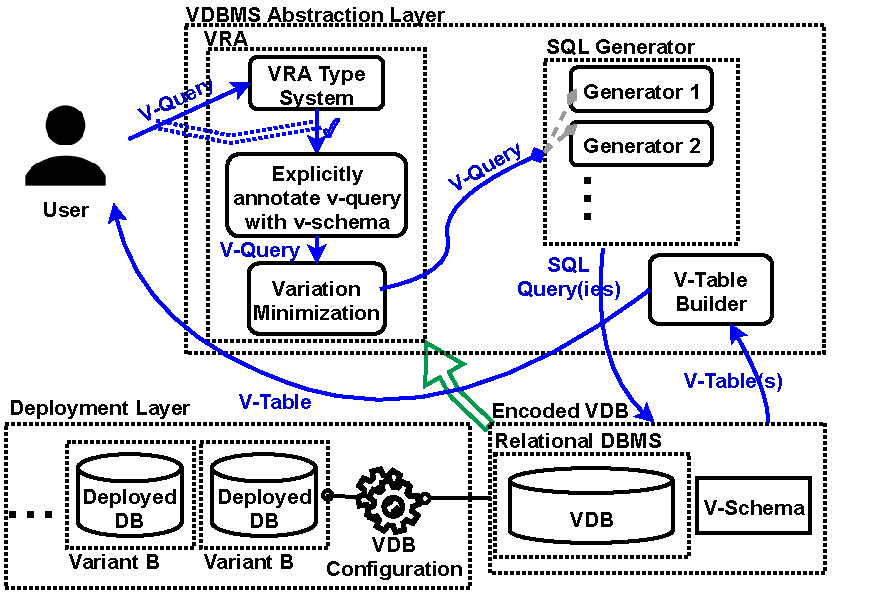
\includegraphics[width = \linewidth] {figs/arch/arch8.pdf}
\caption[VDBMS architecture and execution flow of a variational query]{VDBMS architecture and execution flow of a variational query. 
The dotted double-line from the input variational query
% to explicitly annotate variational query module
indicates the dependency of passing the variational query to this module
only if it is valid. 
The dashed gray arrows with diamond heads demonstrate
an option for the flow of the variational query. 
%We examine taking different routes
%to evaluate a variational query, resulting in various approaches in \secref{apps}.
The blue filled arrows track the data flow, the green hollow arrows 
indicate an input to a module.}
\label{fig:arch}
\end{figure}


%\point{flow of vq in vdbms.}
%Given a VDB and its variational schema, 
To extract information from a VDB, 
a user inputs a variational query \vQ\ to VDBMS.
%
First, \vQ\ is checked by the \emph{type system}.
%, explained in 
%First, \vQ\ is type-checked by the VRA type system introduced in 
%\secref{type-sys}. 
If the query is ill-typed, the user gets an error explaining what part of the 
query violated the variational schema.
%, shown in \exref{q-violate-sch}.
%\moredet{maybe give an ex of an error user will see! ref to ex of error given
%in \secref{type-sys}}
Otherwise, 
\vQ\ is explicitly annotated by the schema and
%defined in \secref{constrain},
%to ensure variation-preserving property w.r.t. variational schema throughout the execution flow of variational query 
%in the system and then
%
%Then, it 
is passed to the \emph{variation minimization} module,
% introduced in 
%\secref{var-min}, 
to simplify \vQ.
%minimize the variation of \vQ\ and apply
%relational algebra optimization rules. 
%
The simplified query is then sent to the \emph{generator} module where
SQL queries are generated from variational queries by different approaches explained 
in \secref{apps}.
%, \secref{apps} provides three
%approaches for this.
%\TODO{
%\exref{q-flow} in \appref{sql-gen} demonstrates the flow of a variational query through
%VDBMS.}
%\wrrite{have examples for each approaches. of mainly the final sql}

\begin{comment}
To generate runnable queries w.r.t. the underlying DBMS,
the minimized query \ensuremath {\VVal \vQ} is passed to 
the \emph{translate to RA} module that could use either 
configuring or grouping of variational queries, explained in \secref{vra-sem},
to generate RA queries. The generated 
queries are then sent to the \emph{SQL generator} module which generates
SQL queries in various ways from the relational algebra queries, explained
in \secref{sql-gen}.
%\moredet{in app have an ex of all this happening!}
\end{comment}

%\point{vtab builder.}
%Having generated a/multiple SQL query/ies, it/they is/are now run over the underlying 
%VDB.
All generated SQL queries are then executed on the underlying VDB.
% (stored in a DBMS desired by the user). 
 The result could be either 
a variational table or multiple variational tables, depending on the approach chosen by
%the translator to RA and 
the SQL generator. The variational table(s) is passed
to the \emph{variational table builder}
%\dropit{could drop \secref{vtab-build} and explain it here!}
%explained in \secref{vtab-build}, 
to create one variational table that filters out 
duplicate and invalid tuples, shrinks presence conditions, and 
eventually, returns the final variational table to the user.
Note that the variational table builder module uses the accumulation
functions introduced in \secref{accum} in addition to filtering out tuples and 
cleaning a variational table. 


%\input{sections/sqlGen}

